\documentclass[../main.tex]{subfiles}
\graphicspath{{\subfix{../Images/}}}
\begin{document}

%\section{Compute Hardware and Network} \label{sec:Atlas_LAN}

Minion distributes processing tasks across multiple computing nodes to achieve real-time performance and robust system operation.
The computing infrastructure consists an embedded computer integrated with the camera sensors for video encoding and streaming, and twin computers serving as the primary processing platforms, with a \ac{GbE} \ac{LAN} connecting all systems and sensors. 
% This architecture distributes computational workloads according to sensor proximity and processing requirements while maintaining centralized coordination through the Robot Operating System middleware. 
The following subsections detail the hardware specifications, system architecture, and network infrastructure that enable real-time multi-modal perception for maritime object detection and sensor fusion.

%%%%%%%%%%%%%%%%%%%%%%%%%%%%%%%%%%%%%%%%%%%%%%%%%%%%%%%%%%%%%%%%%%%%
\subsection{Camera Enclosure} \label{comp:camera_enclosure}

% # Camera Enclosure Computing Platform

The camera enclosure serves as the integrated perception module for the vessel, and was designed as a self-contained sensor and computing subsystem that can operate independently on any maritime or ground vehicle. 
Integrated into this subsystem is a NVIDIA Jetson AGX Xavier, a compact and capable PC designed for video processing, as well as other computer vision applications.
Key hardware specifications are provided in table \ref{table:Xavier_hardware}.

Its 8-core ARM processor provides ample computational capacity for handling multiple video pipelines, network protocols, and system-level services, while the integrated 512-core Volta GPU performs hardware-accelerated video encoding required for concurrent high-resolution streams.  
A unified memory architecture shares 32 GB between the CPU and GPU and supports a memory bandwidth of 136.5 GBps, which minimizes latency and improves overall pipeline efficiency.

Each video feed follows a two-branch processing pipeline before being transmitted to Atlas, detailed in section \ref{time_sync_cam}.

Raw video frames are received via USB 3.0, parsed by custom software, and then split into two processing branches. 
One branch is compressed and saved locally to the Jetson's internal storage, while the other branch is down-sampled to a reduced frame rate before being streamed over the \ac{LAN}.% to one of the Minion PCs in Atlas.





\begin{table}[htpb]
\centering
\begin{tabular}{ll}
\hline
\multicolumn{2}{c}{NVIDIA Jetson AGX Xavier} \\
\hline
% \textbf{Component} & \textbf{Specification} \\
\hline
Processor (CPU) & 64-bit 8-core NVIDIA Carmel \\
Graphics (Integrated) & 512-core NVIDIA Volta \\
Memory (RAM) & 32 GB LPDDR4 \\
Memory Bandwidth & 135 GBps \\
Storage (Primary) & 32 GB eMMC 5.1 \\
Storage (Secondary) & 500 GB NVMe \\
Network Interface & Gigabit Ethernet \\
Operating System & Ubuntu 18.04 \\
\hline
\end{tabular}
\caption{NVIDIA Jetson Xavier - Hardware and Operating System Specifications}
\label{table:Xavier_hardware}
\end{table}

This reduction in frame rate is essential to maintain reliable network performance given limited bandwidth, as discussed in Section \ref{comp:network}. 
The maximum bitrate $R_{\text{max}}$ of each stream is computed at runtime as a function of the target frame rate, frame resolution, and compression ratio, defined by

\begin{equation}
    R_{\text{max}} = N_x N_y b f
\end{equation}

where $N_x$ and $N_y$ are the image width and height in pixels, $f$ is the desired frame rate, and $b$ is the effective bits per pixel after compression.
For the HDR camera, the image resolution is $2880 \times 1860$ pixels, encoded in YUV 4:2:0 format using H.264 compression.
An empirically derived constant of $b = 0.14$ bits per pixel captures the combined effects of color subsampling and compression efficiency under typical scene conditions.
These values yield a bitrate for the HDR camera of
\begin{equation*}
    \begin{split}
        R_{\text{max}} & = (2880 \times 1860\; \text{px}) (0.14 \;\text{bits/px})(5\;\text{s}^{-1})  \\
        & \approx 3.75\; \text{Mbps}
    \end{split}
\end{equation*}

and scales linearly with frame rate.
This adaptive bitrate approach ensures that each video stream remains within the available network bandwidth while maintaining adequate visual fidelity for perception and data logging.
By default, each camera operates at 5 \ac{fps}, aligning with the data rate of other perception sensors, but this rate can be adjusted as needed. % to accommodate specific mission or testing requirements.



While compressed video is streamed to Atlas, the Jetson simultaneously records each feed at its native frame rate to the onboard 500 GB solid-state NVMe drive as redundant backups. 
Each recording is saved in 120-second segments along with a corresponding \ac{CSV} file pairing every image frame with a timestamp from the system clock. 
The same system clock provides the \ac{PTP} signal used by the Livox LiDAR units. ensuring consistent temporal alignment across all sensors within the perception suite. 
Consequently, the timestamps in the recorded \ac{CSV} files are also essential for validating the synchronization of the camera and LiDAR, as discussed in Section \ref{time_sync_cam}.



%%%%%%%%%%%%%%%%%%%%%%%%%%%%%%%%%%%%%%%%%%%%%%%%%%%%%%%%%%%%%%%%%%%%
\subsection{Atlas} \label{atlas}

The primary computing infrastructure consists of two identical high-performance workstation computers, designated Minion A and Minion B.  
Built with enterprise-grade components, these systems provide the computational resources required for real-time sensor processing, object detection, and autonomous navigation.
Table~\ref{table:Minion_hardware} summarizes the key system specifications.
The dual-computer configuration enables parallel software development and operational redundancy, with one system dedicated to production tasks while the other supports software testing or serves as a backup.
 

Each Atlas PC is equipped with computing hardware selected to meet the real-time requirements of multimodal perception and autonomous operation.  
The Intel Xeon processor features six cores and twelve parallel threads that support concurrent execution of perception and navigation processes.  
Tasks requiring low-latency response, such as LiDAR point-cloud filtering and sensor updates, benefit from the processor’s strong single-thread performance, while the multi-core architecture efficiently handles computationally intensive workloads.  
Hardware vector acceleration further enhances numerical operations common to point-cloud transformations and coordinate-frame calculations.

The system’s 16 GB of high-bandwidth DDR4 memory provides sufficient capacity to buffer LiDAR point clouds, video imagery, and navigation data, while offering the throughput necessary for their continuous exchange between processing threads.  
This configuration ensures that shared data structures remain accessible without introducing latency, maintaining consistent performance during extended autonomous operation. 
% This configuration ensures that shared data structures remain accessible across multiple processing threads without introducing latency, maintaining consistent timing performance during extended autonomous operation.

\begin{table}[htpb]
\centering
\begin{tabular}{ll}
\hline
\multicolumn{2}{c}{Minion PC - Hardware Specification} \\
\hline
\hline
Processor (CPU) & Intel Xeon E5-1650 v3 \\
CPU Cores & 6-core / 12-thread, 3.50 GHz \\
Graphics (GPU) & NVIDIA GeForce GTX 1080 \\
GPU Memory & 8 GB GDDR5X, 2560 CUDA cores \\
Memory (RAM) & (4x) 4 GB DDR4 \\
Storage (Primary) & 500 GB NVMe SSD \\
Network Interface & (6x) Gigabit Ethernet \\% + 802.11ac WiFi \\
\hline
\end{tabular}
\caption{Minion A/B PC Hardware Specifications}
\label{table:Minion_hardware}
\end{table}


The GPU is Atlas's primary processor for the system’s vision pipeline, handling both video decoding and neural network inference for object detection.
Each GTX~1080 features 2,560 CUDA cores built on NVIDIA’s Pascal architecture with 8~GB of GDDR5X memory, providing the computational throughput required for highly parallel image-based workloads.  
  
Incoming video streams from the camera enclosure are first decoded using hardware-accelerated video codecs, enabling efficient processing of multiple high-resolution feeds.
The resulting frames are again passed to the GPU for accelerated tensor calculations and neural network based algorithms described in Chapter \ref{realtime_object_detection} for object detection.
% NVIDIA's CUDA architecture has long been the industry standard for efficient execution of convolutional neural networks such as YOLOv8.
Executing both video decoding and inference workloads on the GPU frees up valuable system resources for LiDAR processing and sensor fusion tasks.

High-speed solid-state storage provides the throughput required to record multiple sensor streams during data collection operations.
Each recording session captures raw \ac{LiDAR} point cloud data, streamed video imagery, GPS/INS pose information, and mapped object-detection results, producing aggregate data rates that can easily exceed 200 \ac{MBps}.
A solid-state NVMe hard drive is used on each Minion system to provide the data throughput that these operations require, and is much more robust to the motion experienced in choppy surf and vibrations experienced while in transport on the \ac{USV}'s trailer.


%%%%%%%%%%%%%%%%%%%%%%%%%%%%%%%%%%%%%%%%%%%%%%%%%%%%%%%%%%%%%%%%%%%%
\subsection{Network Structure} \label{comp:network}

% Each device on the network 
Each device is assigned a static IP address on the network, allowing deterministic communication between endpoints.
Camera streams from the Jetson Xavier, point cloud data from each LiDAR sensor, and other telemetry are transmitted over the LAN to Atlas, where sensor data are processed locally.
Data of mapped and detected objects and other system commands, such as motor control commands, are published along with the raw data as \ac{ROS} message topics for system monitoring and data recording.

Under normal operation, the combined network traffic only utilizes about 15\% of the Gigabit Ethernet capacity, 
leaving sufficient headroom for motor control, system services, and remote access for administrative functions.
However, when \ac{ROS} data-dense topics such as point clouds or imagery are broadcast across the network for visualization or debugging, bandwidth utilization can temporarily spike and saturate the network.
For this reason, ROS data is recorded locally, and admin visualization tools such as RVIZ are typically restricted to smaller topics related to object mapping and system controls.
A high-level overview of network utilization is provided in Table \ref{table:network_bandwidth}.

\begin{figure}[htbp]
\centering
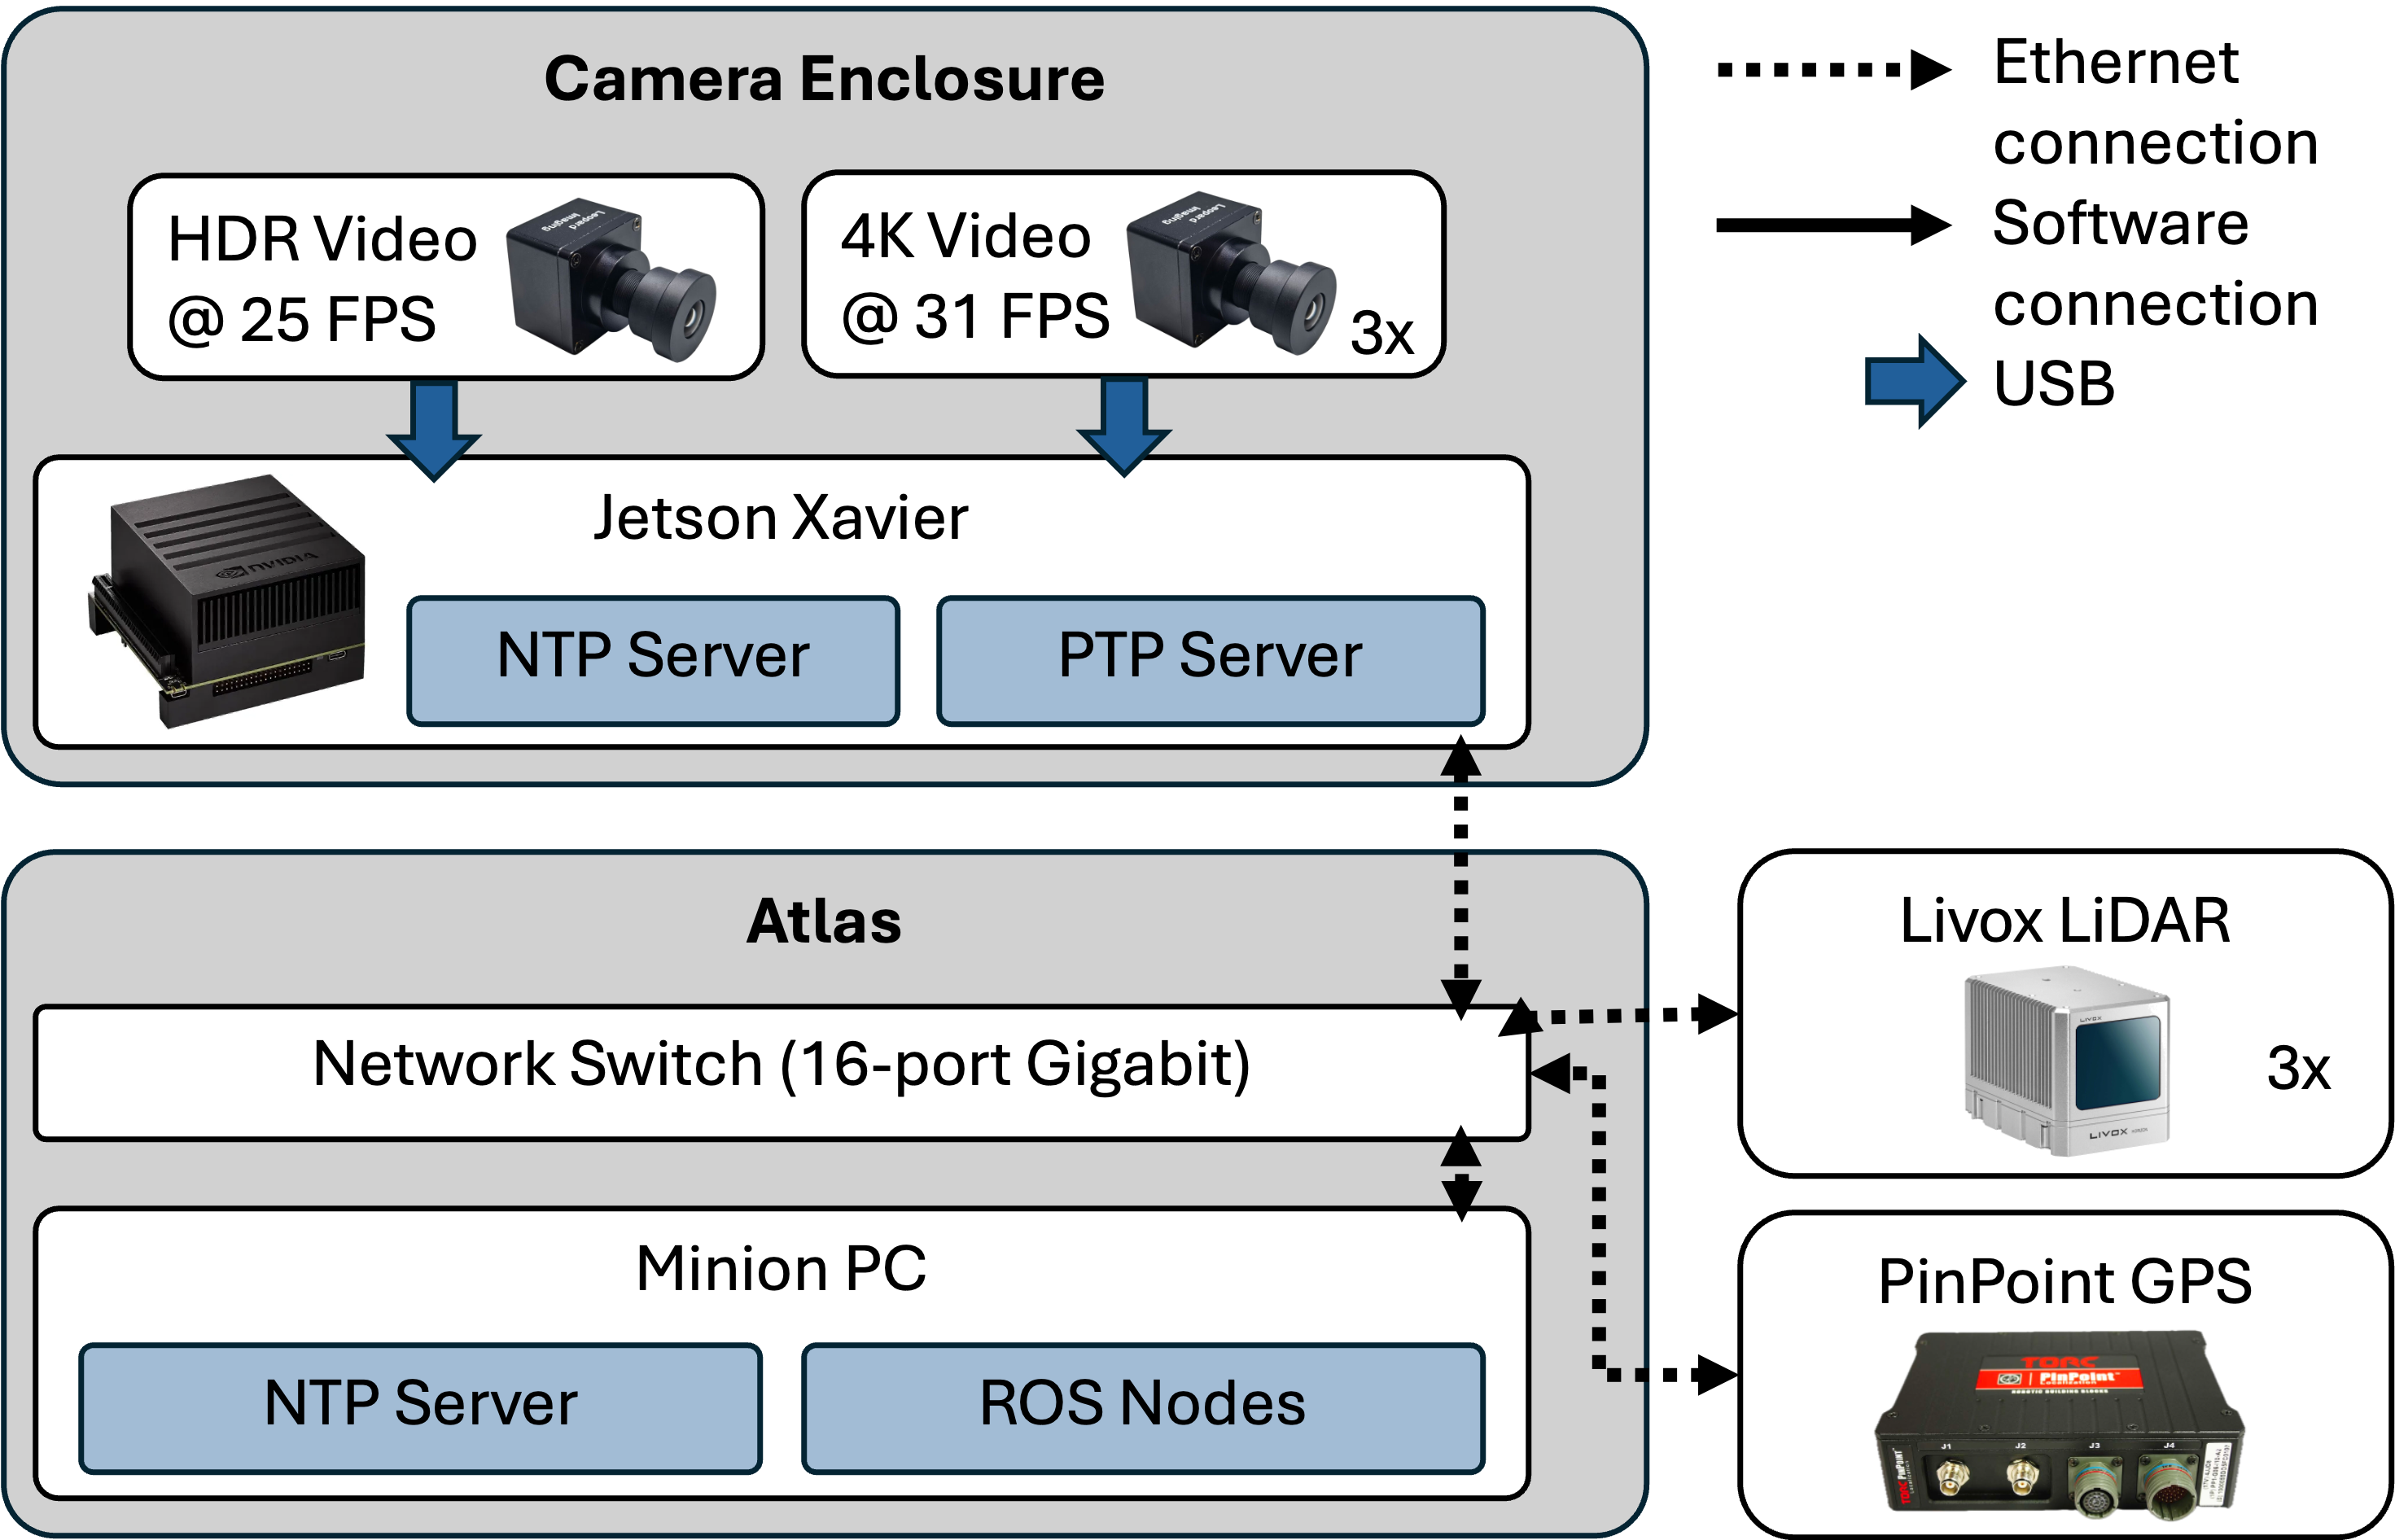
\includegraphics[width=0.8\textwidth]{Images/network_diagram2.png}
\caption{LAN diagram for Minion USV}
\label{fig:network_diagram}
\end{figure}

Although the LAN is primarily dedicated to perception and data logging, it also supports administrative access for configuration, diagnostics, and remote operation.
The Jetson Xavier is configured as a headless device and is accessed remotely via Secure Shell (SSH) for camera configuration, operation, and monitoring.
Each Minion PC can be accessed through SSH for terminal access for development tasks or troubleshooting, or Virtual Network Computing (VNC), and Remote Desktop Protocol (RDP) for a full desktop environment for system administration.
% Network security is intentionally lightweight for field deployment, relying on standard \texttt{sudo}/root authentication and a secured wireless link protected by a strong \ac{WAN} password.
Long-range connectivity between the vessel and ground station is provided by a Ubiquiti Bullet omnidirectional antenna on the \ac{USV}, paired with a directional antenna and a Ubiquiti Dream Machine at the ground station for remote system access and monitoring.

\begin{table}[htbp]
\centering
\begin{tabular}{lcc}
\hline
Data Source & Typical Bandwidth (Mbps) & \% Total Bandwidth \\
\hline
\hline
HDR Camera Stream & $3.7$--$11.2$ & $0.4$--$1.2$ \\
FLIR Camera Streams (2×) & $7.0$--$20.0$ & $0.7$--$2.1$ \\
Velodyne LiDAR Units (3x) & $43.2$--$57.6$ & $4.3$--$5.8$ \\
Livox LiDAR Units (3x) & $40.3$--$53.8$ & $4.0$--$5.4$ \\
GPS / INS Telemetry & $<0.1$ & $<0.01$ \\
Admin / SSH / Control Traffic & $0.5$--$2.0$ & $0.05$--$0.2$ \\
\hline
\textbf{Total Estimated Utilization} & \textbf{95--145 Mbps} & \textbf{9.5--14.5 \%} \\
% \hline
\end{tabular}
\caption{Approximate network bandwidth utilization from direct sensor and control data sources relative to a 1 Gbps link ($\sim940$ Mbps usable).}
\label{table:network_bandwidth}
\end{table}



\end{document}
